\chapter{Spiegel AI Remote}
\textit{Erarbeitet von David Vollmer.}
\\ \\
Im folgenden wird die \textbf{Spiegel AI Remote} App - auch \textbf{Remote App} genannt - beschrieben. Es handelt sich dabei um eine mobile Anwendung, dessen Hauptaufgabe die Fernsteuerung des Smart Mirrors ist.

\section{Funktionen}
Um das Display des Spiegel AIs fernzusteuern, müssen einige Hauptfunktionalitäten vorhanden sein. Die Remote App muss in der Lage sein, mit dem Spiegel zu kommunizieren, die Anzeige der Widgets auf dem Display zu ändern, verfügbare Widgets auszuwählen und Profile zu verwalten. Mit Ausnahme der ersten Anforderung, welche im Kapitel \textbf{Schnittstelle} näher beschrieben wird, werden all diese Punkte in sogenannten Ansichten (englisch: views) behandelt. Diese kann der Nutzer mithilfe einer Navigationsleiste auswählen.
\begin{figure}[h]
    \centering
    \begin{minipage}[b]{0.25\textwidth}
        \centering
        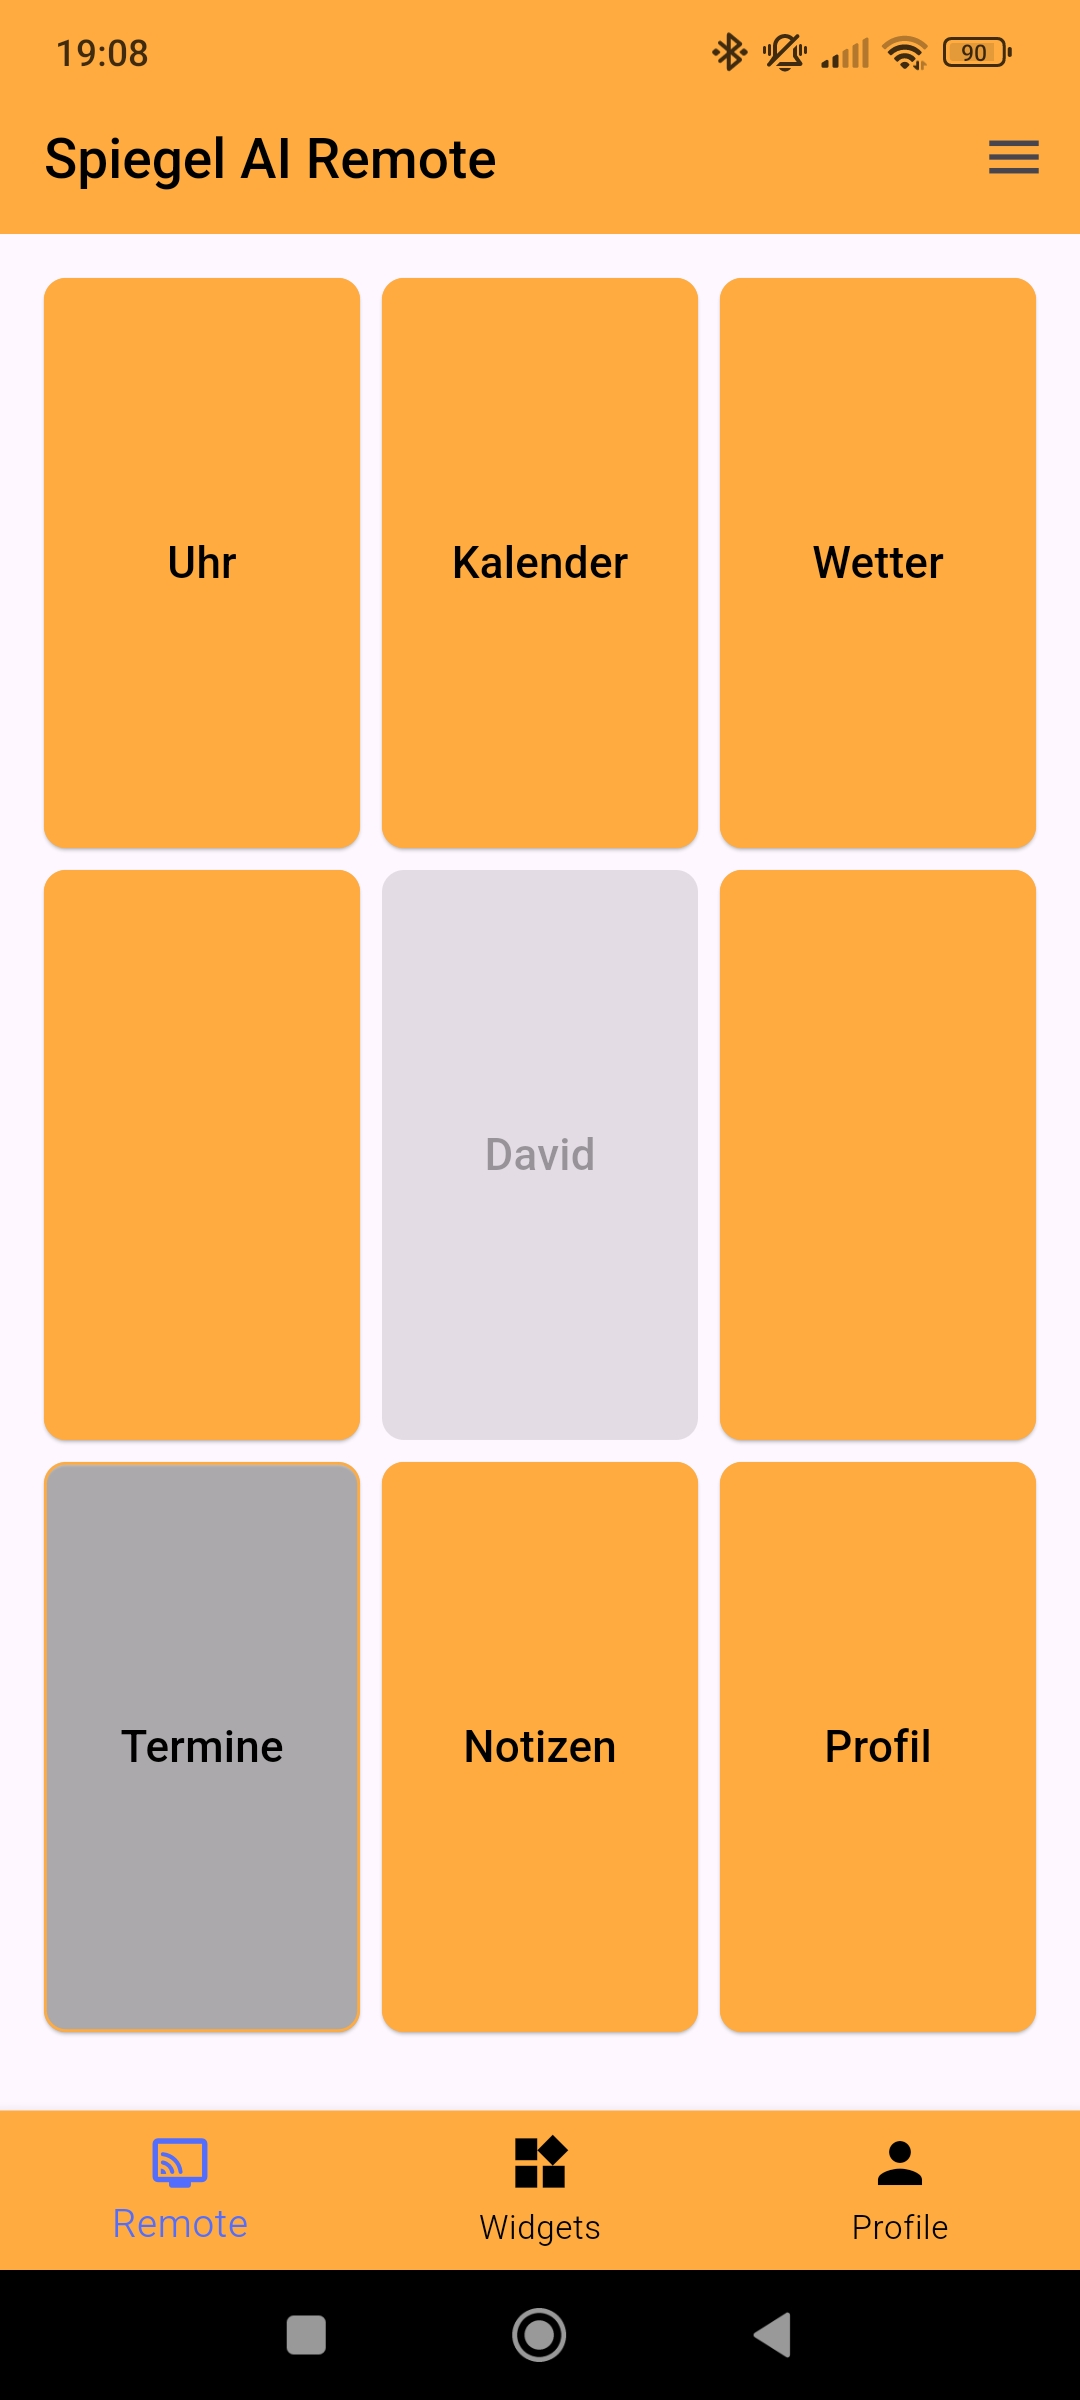
\includegraphics[width=\textwidth]{pictures/remote_remote.jpg}
        \captionsetup{justification=centering, labelformat=simple, singlelinecheck=false}
        \caption{Remote Ansicht\\ Quelle: eigene Darstellung}
    \end{minipage}
    \hfill
    \begin{minipage}[b]{0.25\textwidth}
        \centering
        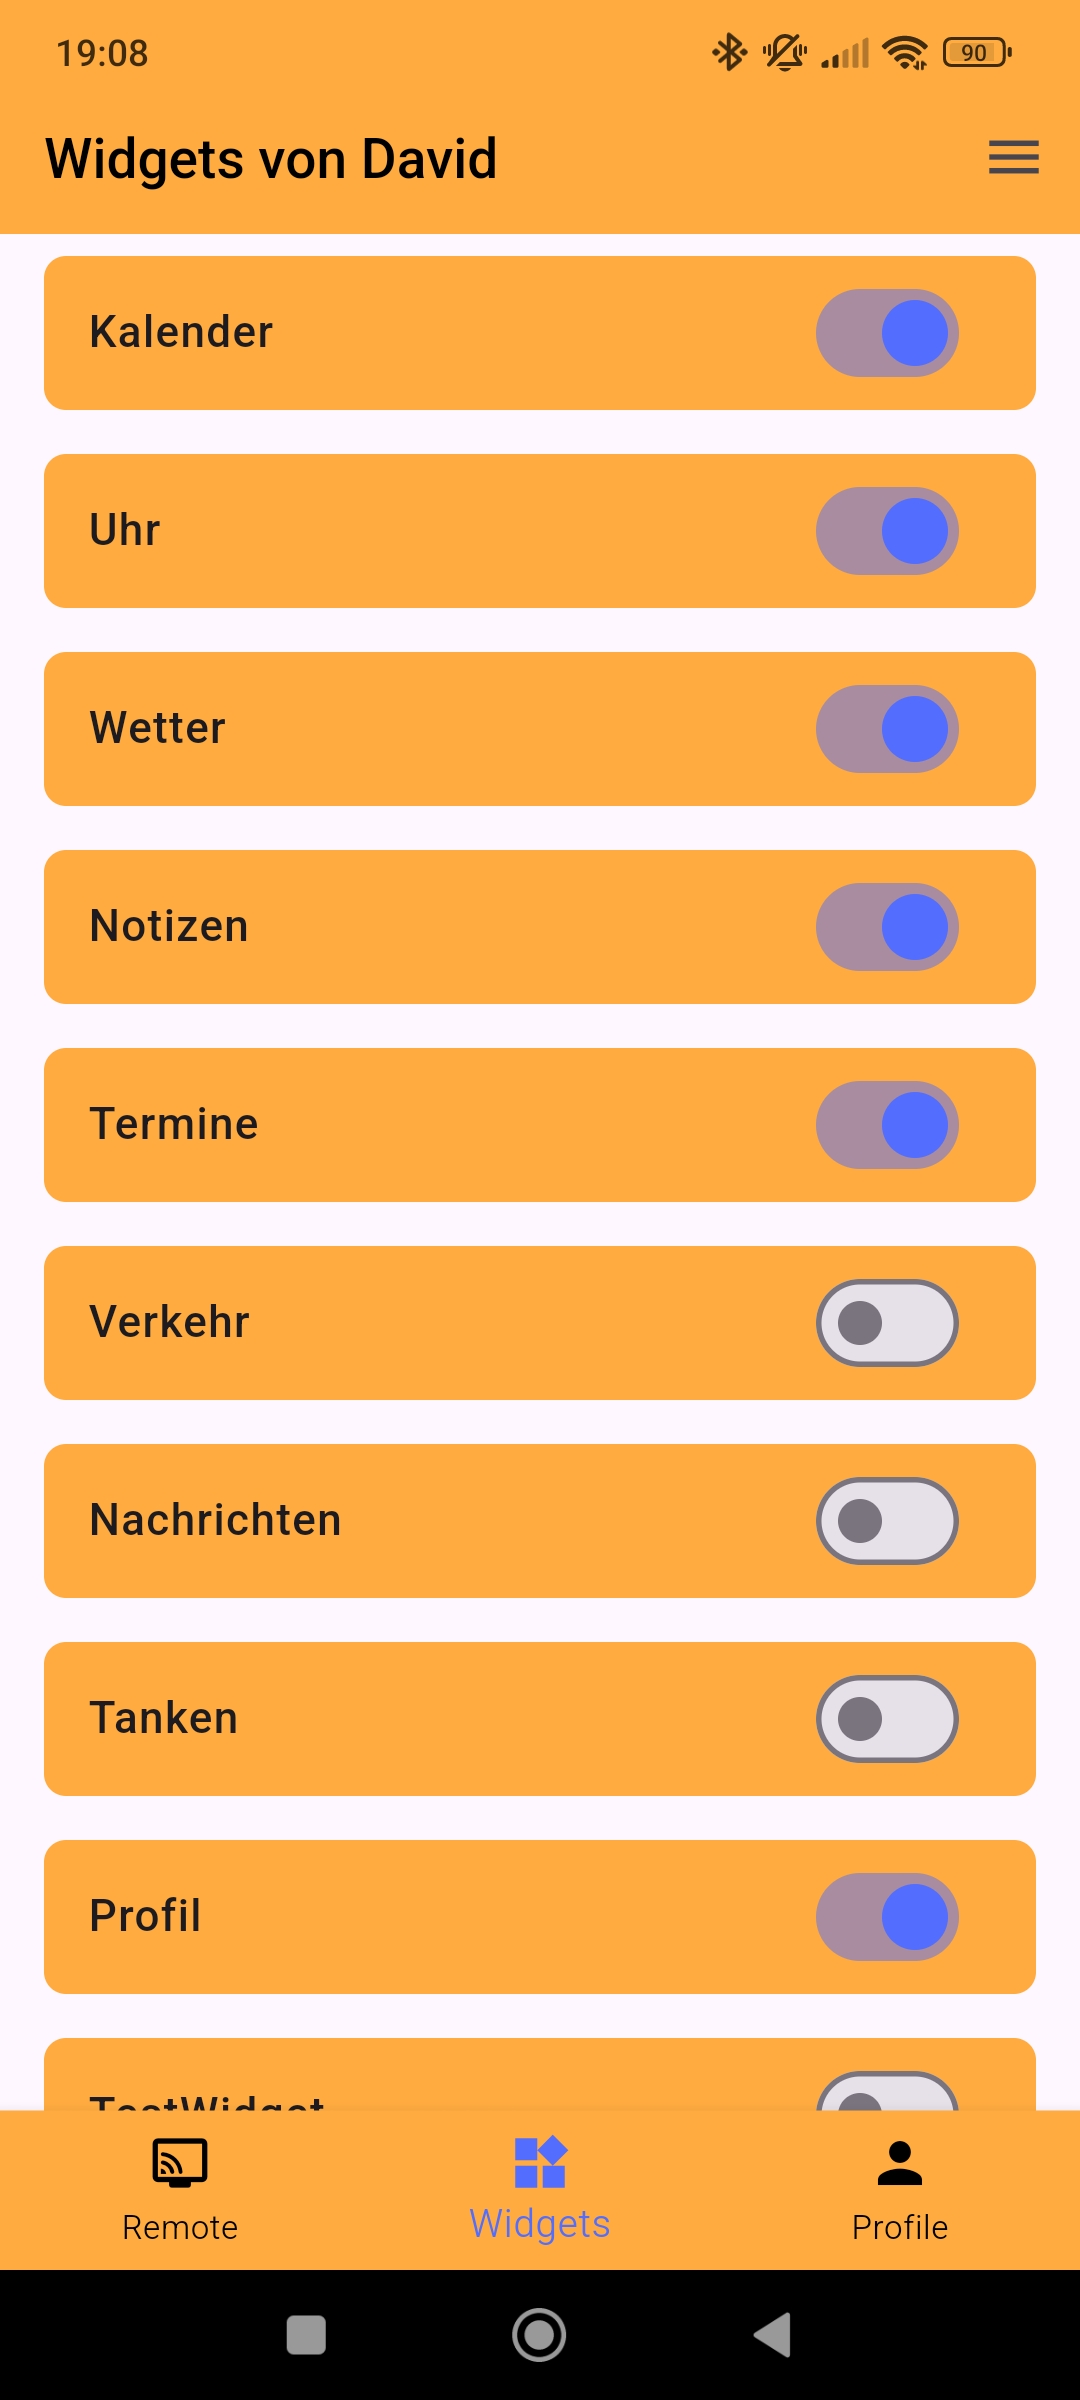
\includegraphics[width=\textwidth]{pictures/remote_widgets.jpg}
        \captionsetup{justification=centering, labelformat=simple, singlelinecheck=false}
        \caption{Widgets Ansicht\\ Quelle: eigene Darstellung}
    \end{minipage}
    \hfill
    \begin{minipage}[b]{0.25\textwidth}
        \centering
        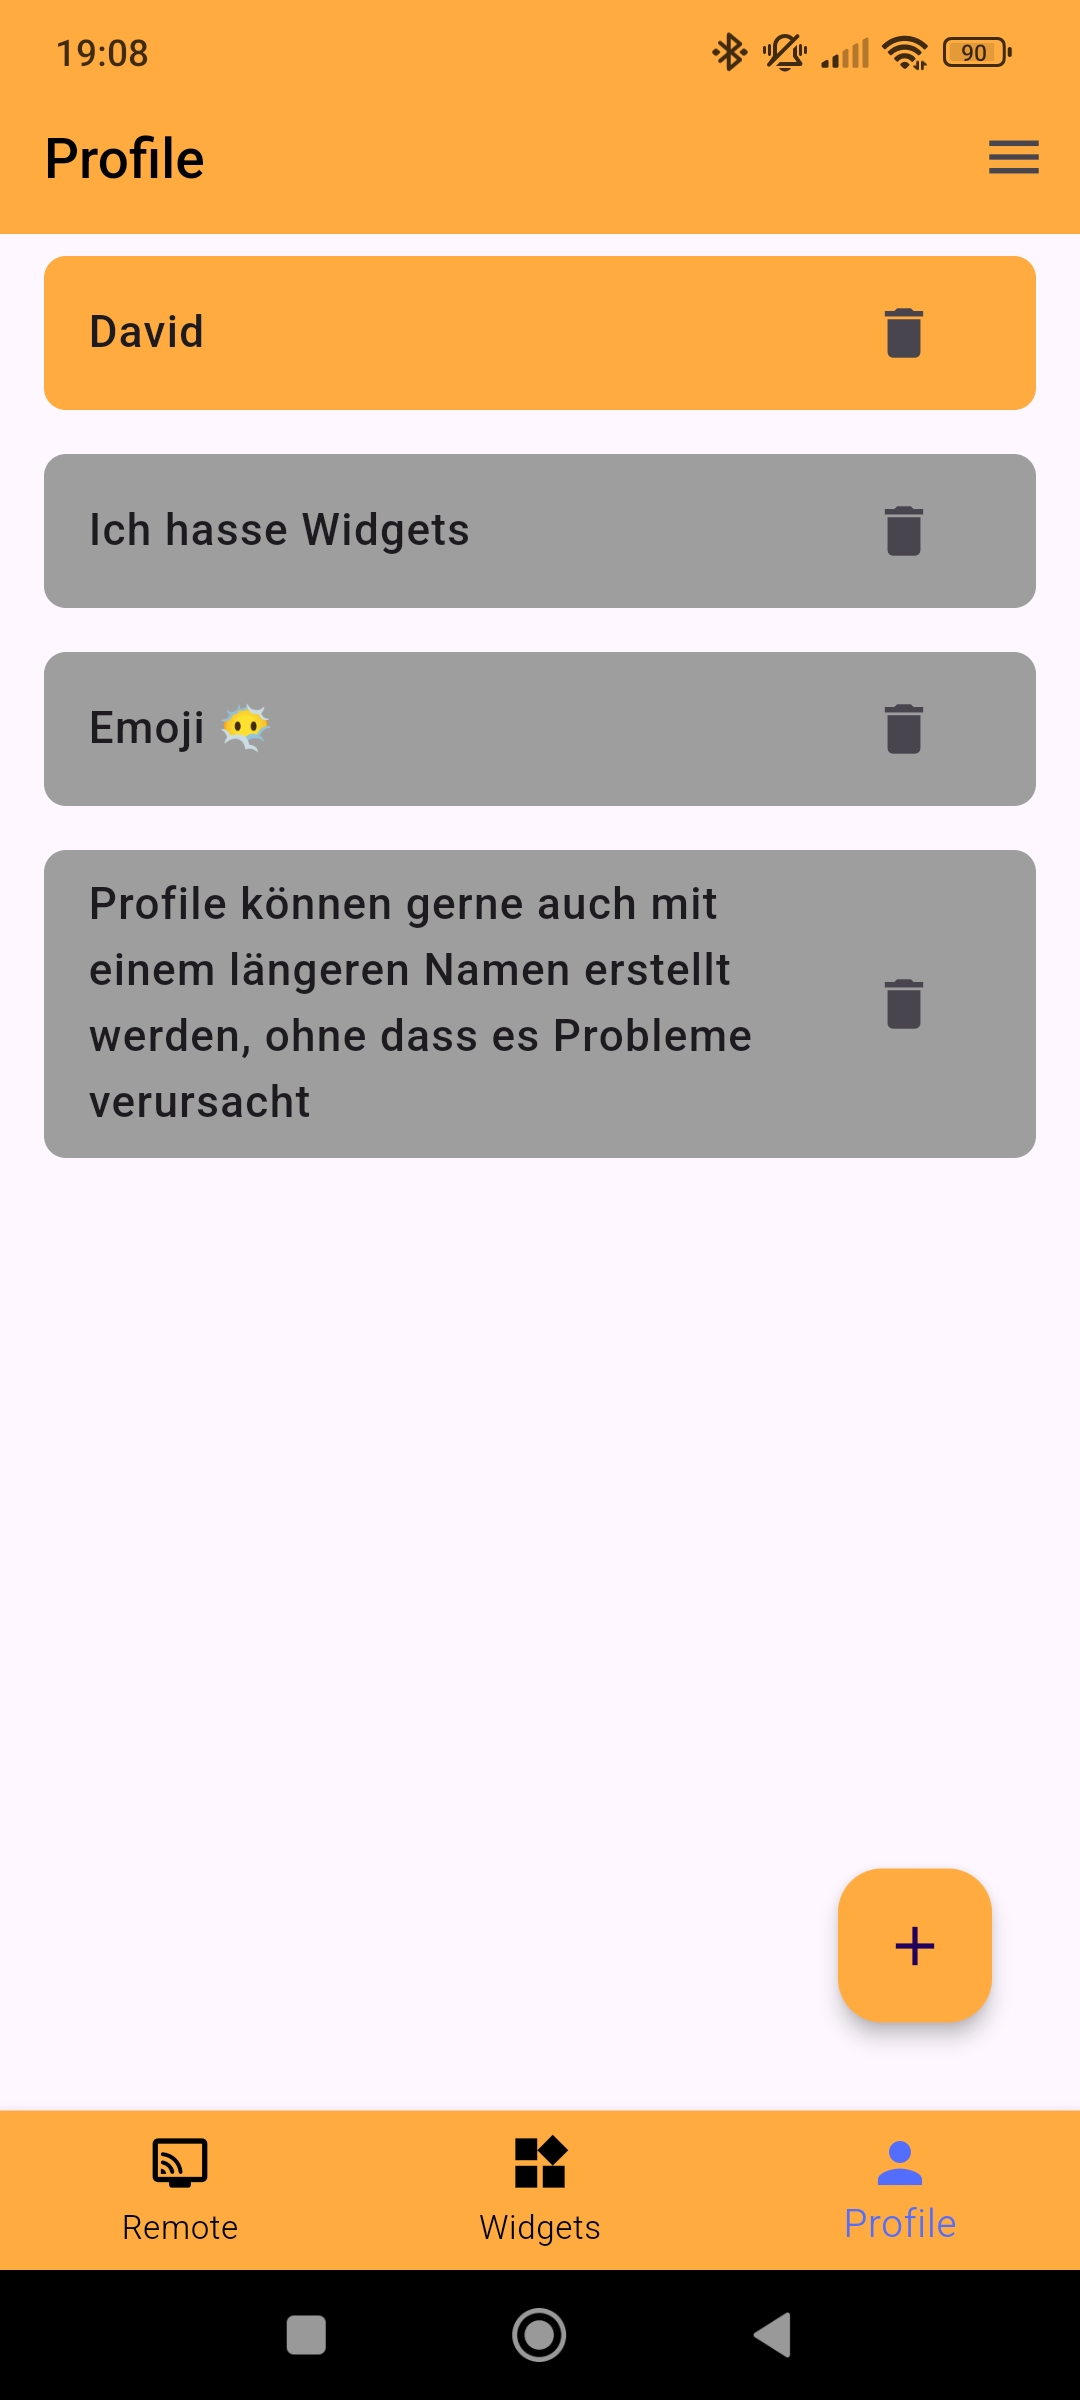
\includegraphics[width=\textwidth]{pictures/remote_profile.jpg}
        \captionsetup{justification=centering, labelformat=simple, singlelinecheck=false}
        \caption{Profile Ansicht\\ Quelle: eigene Darstellung}
    \end{minipage}
\end{figure}

\subsection{Remote View}
Die Remote View, welche die Standardansicht nach Öffnen der App ist, bietet die Möglichkeit, den Status der Displayanzeige am Spiegel zu ändern. In der Mitte wird der Name des gerade ausgewählten Profils angezeigt. Dieses Feld lässt keinerlei Interaktion zu, da das zentrale Feld der Spiegelanzeige frei bleibt. Das bedeutet, dass bis zu acht Widgets angezeigt und geändert werden können. Mit einem Klick auf einen Button wird das jeweilige Widget aus- oder eingeblendet. Ein Feld in grauer Farbe bedeutet, dass das Widget vom Spiegel AI Display nicht angezeigt wird. Zieht man ein Widget über ein anderes, werden ihre Positionen getauscht. Die Felder, die keinen Text enthalten, haben die selben Interaktionsmöglichkeiten wie die anderen. Sie sind Platzhalter für Widgets, die hinzugefügt werden können. Falls kein Profil ausgewählt ist, wird im Remote View eine Standardeinstellung angezeigt und jegliche Interaktion der Buttons ist ausgestellt. Bei einem Versuch, ohne Profilselektion eine Änderung vorzunehmen, wird eine Snackbar angezeigt, welche darauf verweist, dass ein Profil geladen sein muss.

\subsection{Widgets View}
In der Widgets Ansicht können für das ausgewählte Profil Widgets ausgewählt werden. Diese View bietet die Widgets Kalender, Uhr, Wetter, Notizen, Termine, Verkehr, Nachrichten, Tanken, Profil und TestWidget an. Bei letzterem handelt es sich um einen Platzhalter, welcher zum Testen der Widgetfunktionalitäten verwendet wurde, aber auch zukünftig mit einem neuen Widget ersetzt werden kann. Die Anwendungen der restlichen Widgets sind im Kapitel \textbf{Display} beschrieben. Mithilfe eines Toggle-Buttons werden bis zu acht Widgets selektiert. Beim Versuch, ein neuntes Widget auszuwählen, schlägt dies fehl und eine Snackbar benachrichtigt über die Obergrenze erlaubter Widgets. Auf die Änderung eines Widgets, ohne ein Profil geladen zu haben, folgt ebenfalls eine dementsprechende Fehlermeldung. Wird ansonsten ein Widget ausgeschaltet, dann wird das im Toggle-Button signalisiert und in der Remote View wird der Name des Widgets mit einem leeren Feld ersetzt. Wenn ein ausgeschaltetes Widget ausgewählt wird, aktualisiert sich auch da der Toggle-Schalter und in der Remote Ansicht wird das erste Feld ohne Textinhalt mit dem Namen des Widgets versehen.

\subsection{Profile View}
Die letzte navigierbare Ansicht ist die Profile View. Hier findet die Verwaltung der gespeicherten Profile statt. Die Profile werden aufgelistet und können mit einem Klick ausgewählt werden. Hält man ein Profil für eine kurze Zeit gedrückt, kann man diese in ihrer Position in der Auflistung ändern, indem man sie an die gewünschte Stelle zieht. Löschen kann man einen Eintrag, indem auf das Mülleimer-Icon geklickt wird. Darauf öffnet sich ein sogenanntes Alert-Dialog, welches das Abbrechen oder Bestätigen der Löschung durchführt. Ein neues Profil kann erstellt werden, indem auf ein Button, welches sich in der Ansicht rechts unten befindet und mit einem '+'-Symbol gekennzeichnet ist, gedrückt wird. Es erscheint ebenfalls ein Alert-Dialog, welches mithilfe eines Texteingabefeldes einen Profilnamen geben kann. Dieser Prozess kann auch abgebrochen oder bestätigt werden. Falls bei Bestätigung der Name des Profils leer oder schon vergeben ist, wird unterhalb des Textfeldes eine entsprechende Fehlermeldung ausgegeben. Wenn das Erstellen des Profils erfolgreich ist, wird das neue Profil direkt ausgewählt und bekommt die ersten acht Widgets in der Widgets View zugeordnet und werden dementsprechend in der Remote Ansicht angezeigt. Alle Anpassungen, die in diesen beiden Ansichten getätigt werden, werden in den jeweilig ausgewählten Profilen gespeichert.

\section{Implementierung}


\section{Testen}
Testen